\hypertarget{_functionalities_FunctionalitiesDualState}{}\section{Dual State}\label{_functionalities_FunctionalitiesDualState}
A special class should be designed for the framework. Each object of the class has two states for read operation and write operation. The purpose of the class is for thread security. In each cycle, the state of read operation should not be changed. Users can only change the state of write operation. After this cycle, these two states will be synchronised. 
\begin{DoxyImageNoCaption}
  \mbox{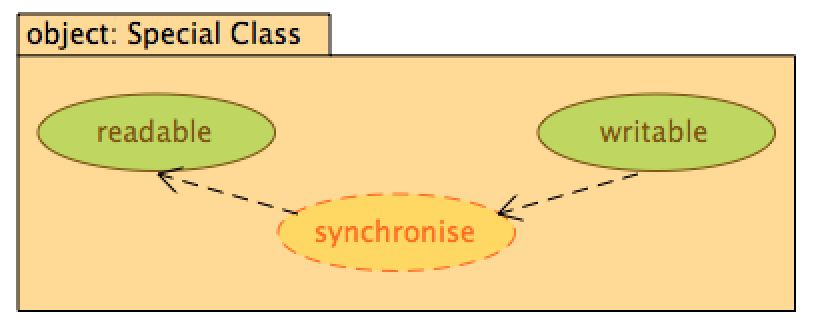
\includegraphics[width=\textwidth,height=\textheight/2,keepaspectratio=true]{FuncSpecDualState.png}}
\end{DoxyImageNoCaption}
\hypertarget{_functionalities_FunctionalitiesMessageDelivery}{}\section{Message Delivery}\label{_functionalities_FunctionalitiesMessageDelivery}
Objects in the framework should be able to send messages to other objects. Each message contains\+: where this message sent from
\begin{DoxyItemize}
\item operation
\item arguments for the operation
\end{DoxyItemize}\hypertarget{_functionalities_FunctionalitiesMailbox}{}\section{Mailbox}\label{_functionalities_FunctionalitiesMailbox}
The mailbox stores messages that object received. It should be designed as Dual State. Therefore, each object will have two copies of mailbox. One is for performing the operation, and the other one is for receiving messages. 
\begin{DoxyImageNoCaption}
  \mbox{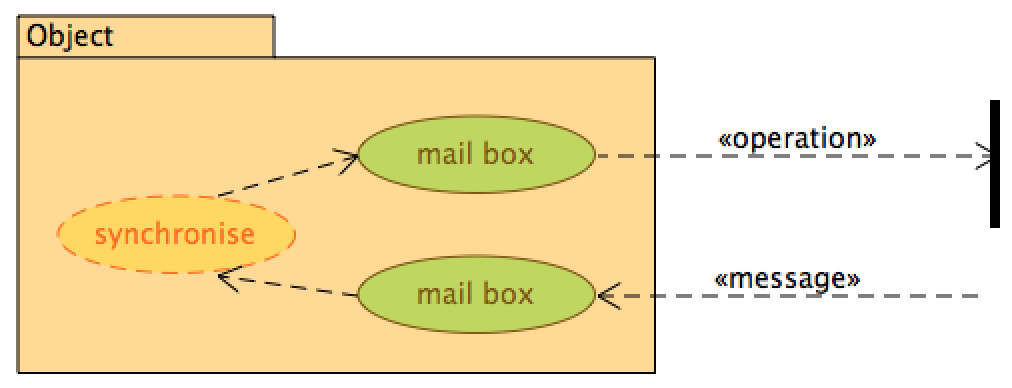
\includegraphics[width=\textwidth,height=\textheight/2,keepaspectratio=true]{FuncSpecMailbox.png}}
\end{DoxyImageNoCaption}
 